\documentclass[11pt]{article}
\usepackage[margin=1in]{geometry}
\usepackage{amsmath,amssymb}
\usepackage{booktabs}
\usepackage{graphicx}
\usepackage{xcolor}
\usepackage[hidelinks]{hyperref}
\usepackage{caption}
\usepackage{parskip}
\usepackage{float}
\usepackage{tabularx}
% generated by train/make_negation_report.py
\newcommand{\PretrainedGreedyRows}{OpenAI GPT-2 124M & \texttt{Paris, and the...} & \texttt{Chicago.} & \texttt{Chicago. There...} & \texttt{Paris.} & \texttt{not Berlin. Th...} \\
GPT-2 + bias (ours) & \texttt{St. Paul, and ...} & \texttt{Chicago.} & \texttt{Chicago. The E...} & \texttt{Paris.} & \texttt{not Berlin.} \\
approach\_3 & \texttt{New York, and ...} & \texttt{Chicago.} & \texttt{Chicago.} & \texttt{Paris.} & \texttt{not Berlin.} \\
three\_residual & \texttt{London, and th...} & \texttt{Chicago.} & \texttt{Chicago. The E...} & \texttt{Paris.} & \texttt{not the capita...} \\
approach\_2 & \texttt{San Francisco,...} & \texttt{Chicago.} & \texttt{Chicago. The E...} & \texttt{Paris.} & \texttt{not Berlin.} \\
approach\_1 (step 3000) & \texttt{the city of th...} & \texttt{Chicago.} & \texttt{Chicago. The E...} & \texttt{Paris.} & \texttt{not Berlin. Th...} \\
approach\_4 & \texttt{} & \texttt{,,,,} & \texttt{the the the th...} & \texttt{,,,,,,,,} & \texttt{the the the th...} \\}
\newcommand{\PretrainedProbRows}{OpenAI GPT-2 124M & 0.070 (\#1) & -- & 0.002 (\#12) & 0.831 (\#1) & 0.001 (\#18) & 0.921 (\#1) & -- & 0.447 (\#1) & 0.129 (\#2) & 0.086 (\#3) \\
GPT-2 + bias (ours) & 0.006 (\#15) & -- & 0.001 (\#66) & 0.501 (\#1) & 0.001 (\#46) & 0.723 (\#1) & -- & 0.585 (\#1) & 0.002 (\#64) & 0.013 (\#8) \\
approach\_3 & 0.006 (\#17) & -- & 0.000 (\#115) & 0.846 (\#1) & 0.000 (\#64) & 0.957 (\#1) & -- & 0.388 (\#1) & 0.003 (\#33) & 0.028 (\#5) \\
three\_residual & 0.019 (\#6) & -- & 0.002 (\#17) & 0.709 (\#1) & 0.001 (\#16) & 0.935 (\#1) & -- & 0.440 (\#1) & 0.004 (\#26) & 0.014 (\#4) \\
approach\_2 & 0.005 (\#16) & -- & 0.001 (\#60) & 0.613 (\#1) & 0.000 (\#66) & 0.820 (\#1) & -- & 0.579 (\#1) & 0.001 (\#132) & 0.004 (\#21) \\
approach\_1 (step 3000) & 0.004 (\#22) & -- & 0.001 (\#75) & 0.308 (\#1) & 0.000 (\#82) & 0.845 (\#1) & -- & 0.210 (\#1) & 0.000 (\#149) & 0.002 (\#20) \\
approach\_4 & 0.000 (\#2756) & -- & 0.000 (\#2190) & 0.000 (\#2591) & 0.000 (\#1320) & 0.000 (\#594) & -- & 0.000 (\#2254) & 0.000 (\#1468) & 0.000 (\#4792) \\}
\newcommand{\FtGreedyRows}{approach\_2, before & \texttt{San Francisco,...} & \texttt{Chicago.} & \texttt{Chicago. The E...} & \texttt{Paris.} & \texttt{not Berlin.} \\
approach\_2, after & \texttt{Toronto.} & \texttt{Toronto.} & \texttt{London.} & \texttt{London.} & \texttt{Paris.} \\
\midrule
GPT-2 + bias (ours), before & \texttt{St. Paul, and ...} & \texttt{Chicago.} & \texttt{Chicago. The E...} & \texttt{Paris.} & \texttt{not Berlin.} \\
GPT-2 + bias (ours), after & \texttt{New York.} & \texttt{New York.} & \texttt{New York. The ...} & \texttt{New York.} & \texttt{Paris.} \\}
\newcommand{\FtMetricRows}{approach\_2, before & 8\% & 6\% & 0\% & 19\% & 22\% & 0\% & 3.675 \\
approach\_2, after & 25\% & 28\% & 28\% & 0\% & 0\% & 100\% & 3.731 \\
\midrule
GPT-2 + bias (ours), before & 17\% & 3\% & 0\% & 19\% & 22\% & 0\% & 3.459 \\
GPT-2 + bias (ours), after & 33\% & 33\% & 36\% & 0\% & 0\% & 100\% & 3.499 \\}
\newcommand{\NHeldLand}{14}\newcommand{\NHeldCap}{22}\newcommand{\NTrainLand}{45}\newcommand{\NTrainCap}{69}
\newcommand{\HeldLandList}{The Golden Gate Bridge, The Acropolis, The Sydney Opera House, Camp Nou, The Bund, The Forbidden City, The CN Tower, Buckingham Palace, The Statue of Liberty, The Rijksmuseum, The Petronas Towers, Anfield, The Gateway Arch, The Grand Ole Opry}
\newcommand{\HeldCapList}{the Philippines, Rwanda, Morocco, Uruguay, Jamaica, Zimbabwe, Serbia, Hungary, Japan, Sweden, Azerbaijan, Malaysia, Italy, Iraq, Venezuela, Sudan, Bangladesh, Chile, Ghana, Jordan, Canada, Croatia}

\newcommand{\code}[1]{\texttt{#1}}
\newcommand{\atwo}{approach\_2}
\newcommand{\base}{GPT-2\,+\,bias}

\title{Can the models answer \code{test\_prompts.txt}?\\
Pretrained checkpoints and a negation fine-tune of approach\_2}
\author{Experiment log, branch \code{attention-experiments}}
\date{2026-10-21}

\begin{document}
\emergencystretch=3em
\maketitle

\section*{Summary}

\code{test\_prompts.txt} asks five questions whose answer is Paris (except P4), most of them preceded by a
negated wrong city:

\begin{tabularx}{\linewidth}{@{}lX@{}}
P1 & The Eiffel Tower is in the city of \\
P2 & The Eiffel Tower is not in Chicago. Therefore, the Eiffel Tower is in the city of \\
P3 & (the sentence ``The Eiffel Tower is not in Chicago.'' six times, then) Therefore, \ldots{} in the city of \\
P4 & The Eiffel Tower is not in Paris. Therefore, the Eiffel Tower is in the city of \\
P5 & The capital of France is not Berlin. Therefore, the capital of France is \\
\end{tabularx}

\begin{itemize}
\item \textbf{No pretrained model answers them.} Every model that trained, including OpenAI's GPT-2 124M,
answers P2 and P3 with the negated city (Chicago, 31--96\% probability) and P4 with Paris. Repeating the
negation (P3) makes them more confident in the wrong city, not less. They copy the city in the prompt rather
than reason about ``not''. \atwo{}, approach\_1, approach\_3 and three\_residual behave the same way as our
GPT-2 baseline; approach\_4, whose pretraining collapsed, emits commas, blank lines or ``the the the''.
\item \textbf{Only OpenAI's GPT-2 knows the fact.} It is the only model with Paris as its top answer to P1
(7\%). Our models, trained on 2.5B tokens, rank Paris 6th to 22nd.
\item \textbf{A 400-step fine-tune removes the copying, but not the missing knowledge.} After fine-tuning
on synthetic ``X is not in D. Therefore, X is in the city of C'' prompts (with Paris, France and the Eiffel
Tower kept out), neither \atwo{} nor \base{} ever answers the negated city on held-out facts (from about
20\%), and their accuracy with a negation equals their accuracy without one. On the test prompts they now
answer P5 correctly (Paris: \atwo{} 44\%, \base{} 97\%), but answer P1--P4 with London, Toronto or New York,
because neither model knows the Eiffel Tower is in Paris.
\item \textbf{\atwo{} learns the skill as well as GPT-2; it just knows fewer facts.} Held-out accuracy after
fine-tuning is 25--28\% for \atwo{} vs 33--36\% for \base{}, the same gap as before fine-tuning on plain
questions, in line with \atwo{}'s higher pretraining loss (3.627 vs 3.405).
\end{itemize}

\section{Models and method}

All checkpoints are the final 2.5B-token OpenWebText runs from the 2026-10-19 and 2026-10-20 reports (the
self-logit bias is annealed to 0, so every model runs as its plain variant). approach\_1 is its step-3000
checkpoint, saved before it diverged. ``\base{}'' is standard GPT-2 124M trained with the same annealed bias,
the control in those reports. OpenAI's pretrained GPT-2 124M is included as a reference: same architecture,
far more training.

For each prompt we record the greedy continuation (8 tokens) and the next-token probability and rank (among
all 50{,}257 tokens) of the correct city and of the city named in the prompt. Script:
\code{train/ask\_prompts.py}.

\section{Pretrained models}

\begin{figure}[H]
\centering
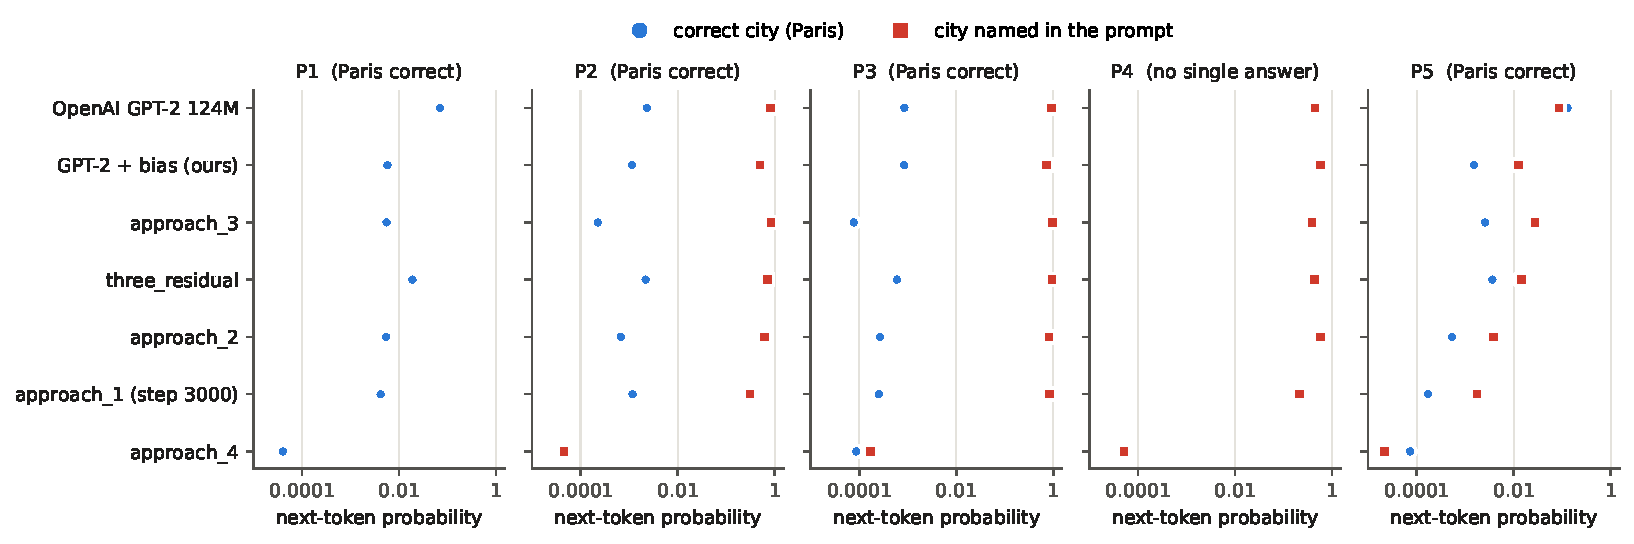
\includegraphics[width=\linewidth]{figures/fig_pretrained_probs.pdf}
\caption{Next-token probability of Paris (blue circle) and of the city named in the prompt (red square:
Chicago in P2--P3, Paris in P4, Berlin in P5). On P2 and P3 every working model puts 30--96\% on Chicago and
under 0.5\% on Paris. Only OpenAI's GPT-2 gives Paris more weight than Berlin on P5.}
\label{fig:pre}
\end{figure}

\begin{table}[H]
\centering
\footnotesize
\setlength{\tabcolsep}{4pt}
\begin{tabular}{@{}lccccc@{}}
\toprule
model & P1 & P2 & P3 & P4 & P5 \\
\midrule
\PretrainedGreedyRows
\bottomrule
\end{tabular}
\caption{Greedy continuation of each prompt (first line, cut at 14 characters).}
\label{tab:pregreedy}
\end{table}

\begin{table}[H]
\centering
\scriptsize
\setlength{\tabcolsep}{3pt}
\resizebox{\linewidth}{!}{%
\begin{tabular}{@{}l*{10}{c}@{}}
\toprule
& \multicolumn{2}{c}{P1} & \multicolumn{2}{c}{P2} & \multicolumn{2}{c}{P3} & \multicolumn{2}{c}{P4} &
\multicolumn{2}{c}{P5} \\
\cmidrule(lr){2-3}\cmidrule(lr){4-5}\cmidrule(lr){6-7}\cmidrule(lr){8-9}\cmidrule(lr){10-11}
model & Paris & -- & Paris & Chicago & Paris & Chicago & -- & Paris & Paris & Berlin \\
\midrule
\PretrainedProbRows
\bottomrule
\end{tabular}}
\caption{Probability (rank) of the correct city and of the city named in the prompt.}
\label{tab:preprob}
\end{table}

Three observations:
\begin{enumerate}
\item \textbf{Copying wins over negation.} In P2--P4 the most likely answer is always the city in the
prompt. This is the known behavior of small language models (``not'' barely changes the next-token
distribution), and the architecture changes do not affect it: all working variants, ours and OpenAI's,
agree on every greedy answer for P2--P4.
\item \textbf{Repetition strengthens it.} Going from one negated sentence (P2) to six (P3) raises
P(Chicago) for every working model, e.g.\ 0.61 $\to$ 0.82 for \atwo{}.
\item \textbf{The fact itself is weak.} On P1 our models put 0.5--2\% on Paris; three\_residual ranks it
6th, the others 15th--22nd. OpenAI's GPT-2 ranks it 1st (7\%). P5 is similar: only OpenAI's GPT-2 prefers
Paris over Berlin.
\end{enumerate}

\section{Fine-tuning approach\_2 to ignore negated cities}

\subsection{Setup}

The question is whether \atwo{} can be taught to ignore a negated distractor, and whether that skill
transfers to facts it was not fine-tuned on. \base{} gets the identical fine-tune as a control.

\paragraph{Data.} Hand-written facts: \NTrainLand{}+\NHeldLand{} landmarks (landmark $\to$ city) and
\NTrainCap{}+\NHeldCap{} countries (country $\to$ capital). Every fact involving Paris, France or the Eiffel
Tower is excluded, so the five test prompts stay unseen. A random 25\% of each list is held out for evaluation:

\begin{itemize}
\item held-out landmarks: \HeldLandList{}.
\item held-out countries: \HeldCapList{}.
\end{itemize}

Each training example uses one of three forms, sampled 1:2:1:
\begin{itemize}
\item plain: ``The Colosseum is in the city of'' $\to$ `` Rome.''
\item negated: ``The Colosseum is not in Oslo. Therefore, the Colosseum is in the city of'' $\to$ `` Rome.''
\item repeated: the negated sentence 2--6 times, then the question.
\end{itemize}
Countries use ``The capital of X is (not D). Therefore, the capital of X is''. The distractor D is a random
other city from the pool of answer cities plus 18 large cities (Chicago among them).

\paragraph{Training.} 400 steps, AdamW ($\beta=(0.9,0.95)$, no weight decay), learning rate $3\times10^{-5}$
after a 20-step warmup, gradient clip 1.0. Each step has 64 synthetic prompts, with the loss on the answer tokens only,
plus 8 OpenWebText sequences of 1024 tokens with the normal language-model loss, to limit forgetting. One run
per model, seed 0, about 1.5 minutes on one GPU. Script: \code{train/finetune\_negation.py}.

\paragraph{Evaluation.} For each entity and form, greedy-decode as many tokens as the answer has. A prompt
is \emph{correct} if the decoded text equals the city, and counts as \emph{answering the negated city} if it starts
with the distractor. OpenWebText loss is measured on the first 64 validation sequences (65k tokens), so it is
comparable before vs after but not to the full-split numbers in earlier reports.

\subsection{Results}

\begin{figure}[H]
\centering
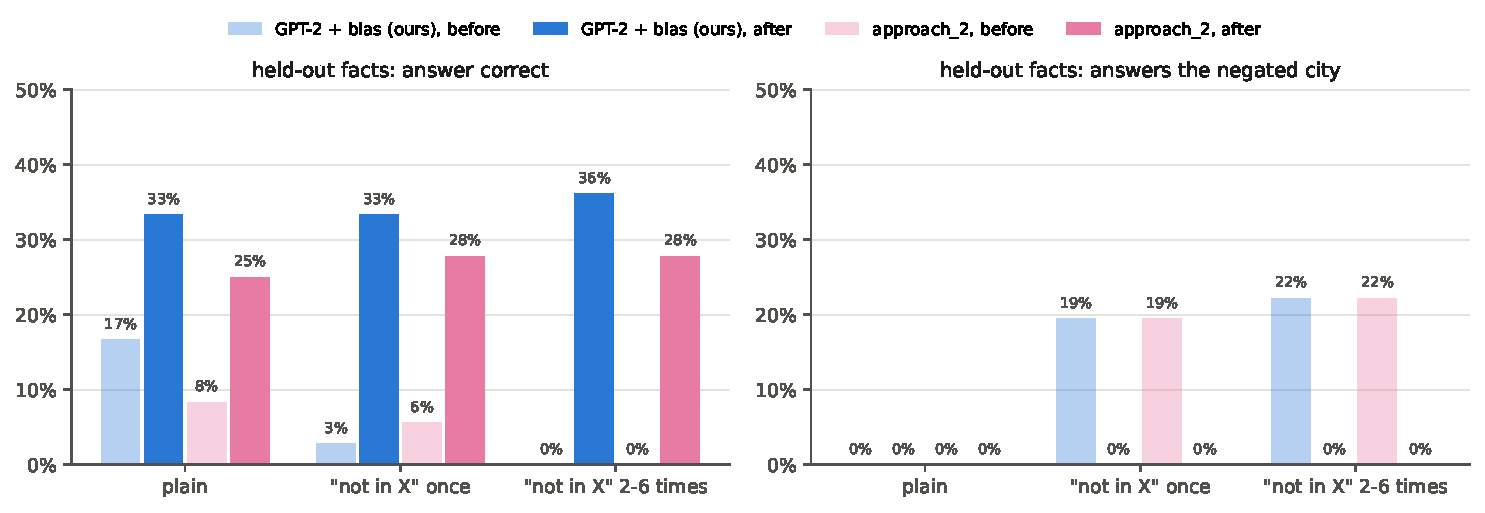
\includegraphics[width=\linewidth]{figures/fig_ft_heldout.pdf}
\caption{Held-out facts (36 entities, so one prompt is 2.8 points), before (faded) and after (solid) fine-tuning.
Left: accuracy. Right: how often the model answers with the negated city.}
\label{fig:fthold}
\end{figure}

\begin{table}[H]
\centering
\small
\begin{tabular}{@{}lccccccc@{}}
\toprule
& \multicolumn{3}{c}{held-out: correct} & \multicolumn{2}{c}{held-out: negated city} & train ents. & OWT \\
\cmidrule(lr){2-4}\cmidrule(lr){5-6}
model & plain & once & 2--6$\times$ & once & 2--6$\times$ & once, correct & loss \\
\midrule
\FtMetricRows
\bottomrule
\end{tabular}
\caption{Fine-tuning metrics. ``once'' and ``2--6$\times$'' are the negated forms.}
\label{tab:ftmetrics}
\end{table}

\begin{itemize}
\item \textbf{The skill transfers to unseen facts.} Before fine-tuning, both models answered the negated city
on about 20\% of held-out negated prompts and were almost never right (0--6\%). Afterwards, they never
answer the negated city, and accuracy is the same with or without the negation (\atwo{}: 25\% plain,
28\% negated; \base{}: 33\% vs 33--36\%). The fine-tune taught ``ignore the negated city'', not just answers.
\item \textbf{Plain-fact accuracy also rose} (\atwo{} 8\% $\to$ 25\%, \base{} 17\% $\to$ 33\%). The question
format and the answer format (a city, then a period) became familiar, so the models now produce knowledge
they already had but did not express.
\item \textbf{Knowledge sets the ceiling, and \atwo{} has less.} \atwo{} trails \base{} by about 8 points
on every form, both before and after, consistent with its higher pretraining loss.
\item \textbf{Cost.} OpenWebText loss rose by 0.056 for \atwo{} and 0.040 for \base{}. The training-entity
answers were memorized (answer loss below $10^{-3}$, 100\% correct), see Figure~\ref{fig:ftcurves}.
\end{itemize}

\begin{figure}[H]
\centering
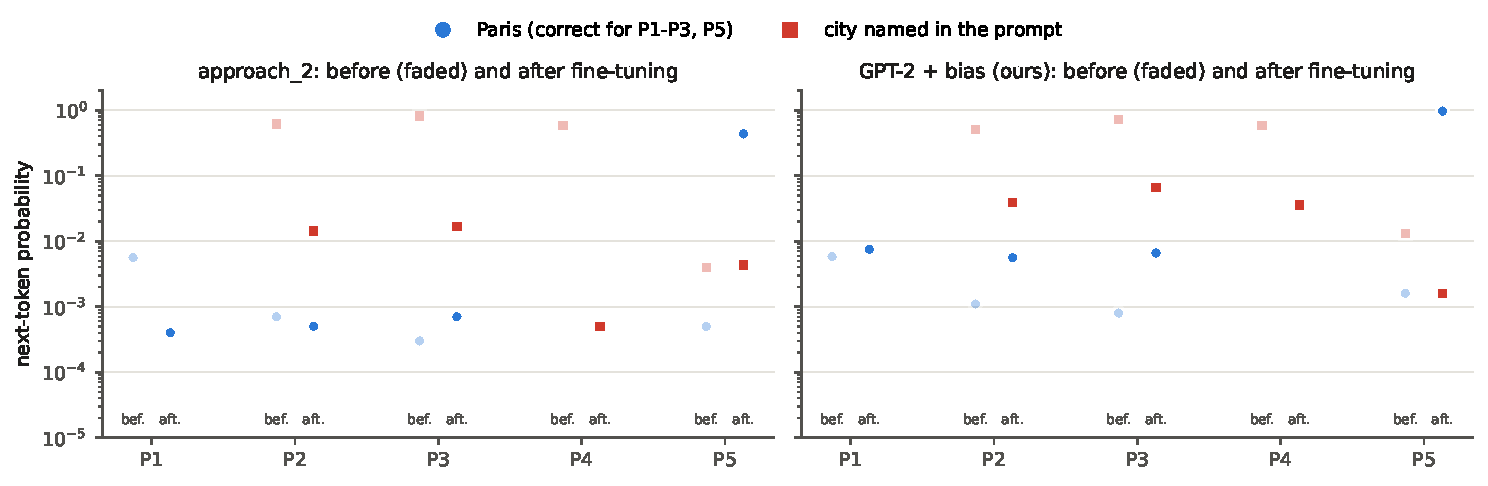
\includegraphics[width=\linewidth]{figures/fig_ft_prompts.pdf}
\caption{Test prompts before (faded) and after fine-tuning. Red squares: the city named in the prompt;
blue circles: Paris.}
\label{fig:ftprompts}
\end{figure}

\begin{table}[H]
\centering
\footnotesize
\setlength{\tabcolsep}{4pt}
\begin{tabular}{@{}lccccc@{}}
\toprule
model & P1 & P2 & P3 & P4 & P5 \\
\midrule
\FtGreedyRows
\bottomrule
\end{tabular}
\caption{Greedy answers to the test prompts before and after fine-tuning.}
\label{tab:ftgreedy}
\end{table}

On the test prompts (Figure~\ref{fig:ftprompts}, Table~\ref{tab:ftgreedy}):
\begin{itemize}
\item \textbf{The copying is gone.} P(Chicago) on P2--P3 fell from 0.5--0.8 to 0.01--0.07, and P4 no longer
answers Paris.
\item \textbf{P5 is solved} by both models (Paris: \atwo{} 0.44, \base{} 0.97), since both know France's capital
once the Berlin distractor is ignored.
\item \textbf{P1--P3 are not.} Both models now answer with a frequent training answer (\atwo{}: Toronto or
London; \base{}: New York). For \atwo{}, P(Paris) on P1 even dropped (0.006 $\to$ 0.0004).
\end{itemize}

The drop has a likely cause in the data design. Paris was never an answer during fine-tuning, while London and New
York were the most frequent answers (4 training entities each), so the fine-tune shifts probability toward those cities.
For a model that does not know the fact, the frequent answers win. \base{}'s P(Paris) on P1--P3 rose slightly
(0.006--0.007 after), but stayed far below its top answer.

\begin{figure}[H]
\centering
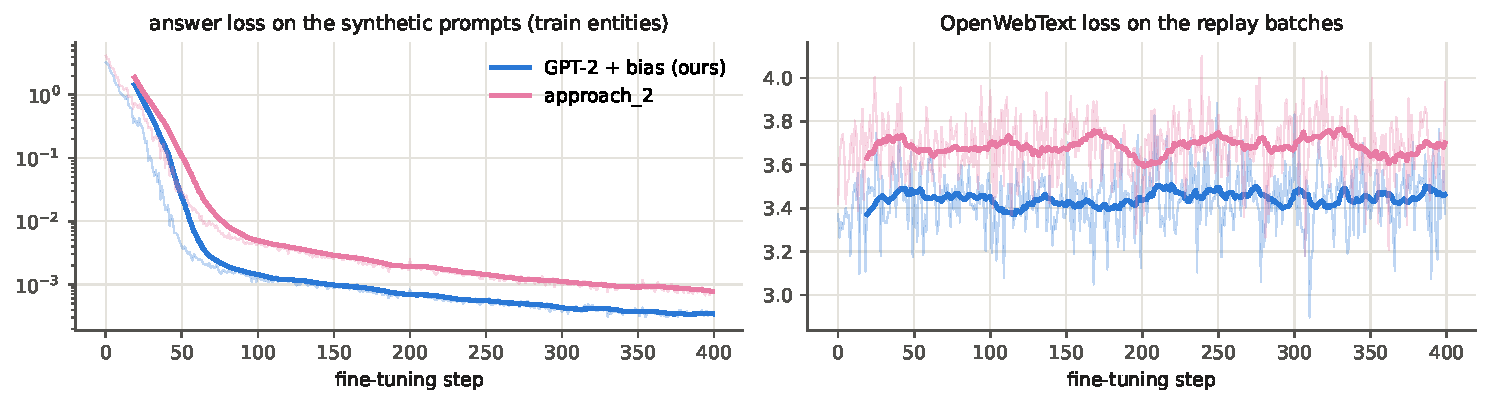
\includegraphics[width=\linewidth]{figures/fig_ft_curves.pdf}
\caption{Fine-tuning curves (thin: per step; thick: 20-step mean). Left: answer loss on the synthetic
training prompts, log scale. Right: loss on the OpenWebText replay batches, which stays at each model's
pretraining level.}
\label{fig:ftcurves}
\end{figure}

\section{Limitations}

\begin{itemize}
\item One seed per configuration, and only 36 held-out entities (108 prompts), so each held-out percentage
is uncertain by roughly $\pm$8 points. The \atwo{} vs \base{} gap after fine-tuning is about one such
interval.
\item The facts list is small and hand-written, and the templates are fixed. The fine-tune likely teaches
this exact phrasing; other forms of negation (``isn't'', ``rather than'') were not tested.
\item Entities are held out, but answer cities are not: a held-out landmark in London has an answer the
fine-tune trained on, which can inflate held-out accuracy. The negated-city rate (20\% $\to$ 0\%) does not
depend on this.
\item Excluding all Paris answers protects the test prompts but biases the models away from Paris (above).
\item P4 has no single correct answer, so it is only used to check that the model stops repeating the city
in the prompt.
\end{itemize}

\section{Possible next steps}

\begin{itemize}
\item Add plain ``The Eiffel Tower is in the city of Paris.'' (and other Paris facts) to fine-tuning, but no
negated Eiffel prompts. P2--P4 would then test only the negation skill, with knowledge out of the way.
\item Mix several negation phrasings and test on unseen ones, to see whether the skill is about ``not'' or
about this template.
\item Fine-tune OpenAI's GPT-2 124M the same way: it already knows the Eiffel Tower fact, so it shows what
the fine-tune achieves when knowledge is not the limit.
\item Repeat with 3 seeds and a larger held-out set to resolve the \atwo{} vs \base{} gap.
\end{itemize}

\section*{Files}

\begin{itemize}
\item \code{data/}: \code{prompts\_pretrained.json} (all pretrained models),
\code{ft\_approach\_2\_results.json} and \code{ft\_baseline\_results.json}
(before/after metrics, entity split, test-prompt outputs), \code{ft\_*\_log.jsonl} (per-step losses),
\code{test\_prompts.txt}.
\item \code{code/}: \code{ask\_prompts.py}, \code{finetune\_negation.py}, \code{make\_negation\_report.py}.
\item Fine-tuned weights: \url{/local/scratch/a/liu3170/runs/openwebtext/ft_negation/approach_2/finetuned.pt}
and the same path with \code{baseline}.
\end{itemize}

\end{document}
